%% LyX 2.3.6 created this file.  For more info, see http://www.lyx.org/.
%% Do not edit unless you really know what you are doing.
\documentclass[english,aspectratio=169]{beamer}
\usepackage{lmodern}
\renewcommand{\sfdefault}{lmss}
\renewcommand{\ttdefault}{lmtt}
\usepackage[T1]{fontenc}
\usepackage[latin9]{inputenc}
\setlength{\parskip}{\medskipamount}
\setlength{\parindent}{0pt}
\usepackage{amsbsy}
\usepackage{amssymb}
\usepackage{cancel}
\usepackage{graphicx}
\PassOptionsToPackage{normalem}{ulem}
\usepackage{ulem}

\makeatletter

%%%%%%%%%%%%%%%%%%%%%%%%%%%%%% LyX specific LaTeX commands.
\pdfpageheight\paperheight
\pdfpagewidth\paperwidth


%%%%%%%%%%%%%%%%%%%%%%%%%%%%%% Textclass specific LaTeX commands.
% this default might be overridden by plain title style
\newcommand\makebeamertitle{\frame{\maketitle}}%
% (ERT) argument for the TOC
\AtBeginDocument{%
  \let\origtableofcontents=\tableofcontents
  \def\tableofcontents{\@ifnextchar[{\origtableofcontents}{\gobbletableofcontents}}
  \def\gobbletableofcontents#1{\origtableofcontents}
}

%%%%%%%%%%%%%%%%%%%%%%%%%%%%%% User specified LaTeX commands.
\usetheme{CambridgeUS}
\usecolortheme{dolphin}
\hypersetup{pdfpagemode=None}
\usepackage{tikz}
\usepackage{color}
\usepackage{listings}

\makeatother

\usepackage{babel}
\begin{document}
\title[M3-4]{The continuity equation}
\author{Department of Oceanography}
\institute[UCT]{University of Cape Town}
\date{SEA3004F}
\makebeamertitle

\section*{Outlines}
\begin{frame}{Outline}

\tableofcontents{}
\end{frame}


\section{Flow in a conduit}
\begin{frame}{Flow in a conduit and incompressibility}

\begin{center}
\vspace{-0.5cm}
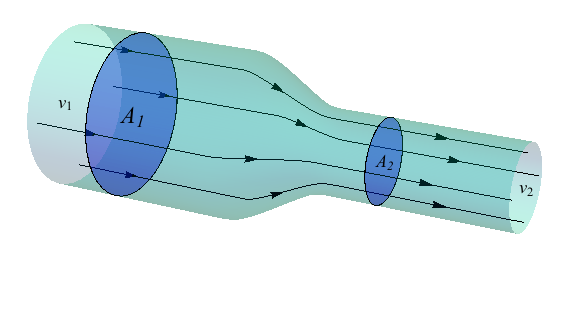
\includegraphics[scale=0.4]{../figures/M3/FluidContinuity}
\par\end{center}
\begin{itemize}
\item \vspace{-1cm}
{\scriptsize{}When water flows through a conduit, we observe that
the velocity depends on the size of the section. Where the section
is large, the velocity is smaller; It increases where the pipe becomes
narrower. This is an indication of the conservation of mass in an
}\textbf{\scriptsize{}incompressible fluid}{\scriptsize{}. The mass
flow rate (expressed in }\textbf{\scriptsize{}mass per unit time}{\scriptsize{})
has to be conserved because the volume of the water must be conserved:
\begin{equation}
\rho_{1}v_{1}A_{1}=\rho_{2}v_{2}A_{2}\label{eq:flow_rate}
\end{equation}
}{\scriptsize\par}
\item {\scriptsize{}The water is incompressible for all practical purposes,
and this is the main approximation done in geophysical fluid dynamics.
(Note that water is compressible to a certain extent otherwise there
would not be any sound propagation) }{\scriptsize\par}
\end{itemize}
\end{frame}


\section{Mass conservation}
\begin{frame}{Mass conservation: Eulerian derivation}

\begin{columns}[t]


\column{7cm}
\begin{itemize}
\item {\scriptsize{}In GFD we need a more general definition of mass conservation
because the flow is not constrained in a conduit. We will derive the
mass conservation equation from an Eulerian point of view: we imagine
a reference volume that is }\textbf{\scriptsize{}fixed in space}{\scriptsize{}
at a certain location $(x,y,z)$, the lower left corner of the box,
and the fluid that flows through it }{\scriptsize\par}
\item {\scriptsize{}The fluid is defined by the Eulerian fields for velocity,
the vector field $\mathbf{u}=\left(u,v,w\right)$, and density, the
scalar field $\rho(x,y,z)$}{\scriptsize\par}
\item {\scriptsize{}We compute the mass flow rate passing through the sides
(in and out) using the concept shown in eq. (\ref{eq:flow_rate}).
The x-component is 
\begin{align*}
Q_{in} & =\left[\rho(x)\,u(x)\right]_{x}\delta y\delta z\\
Q_{out} & =\left[\rho(x+\delta x)\,u(x+\delta x)\right]_{x}\delta y\delta z=\\
 & =\left[\left(\rho+\delta\rho\right)\left(u+\delta u\right)\right]_{x}\delta y\delta z
\end{align*}
} 
\end{itemize}

\column{7cm}

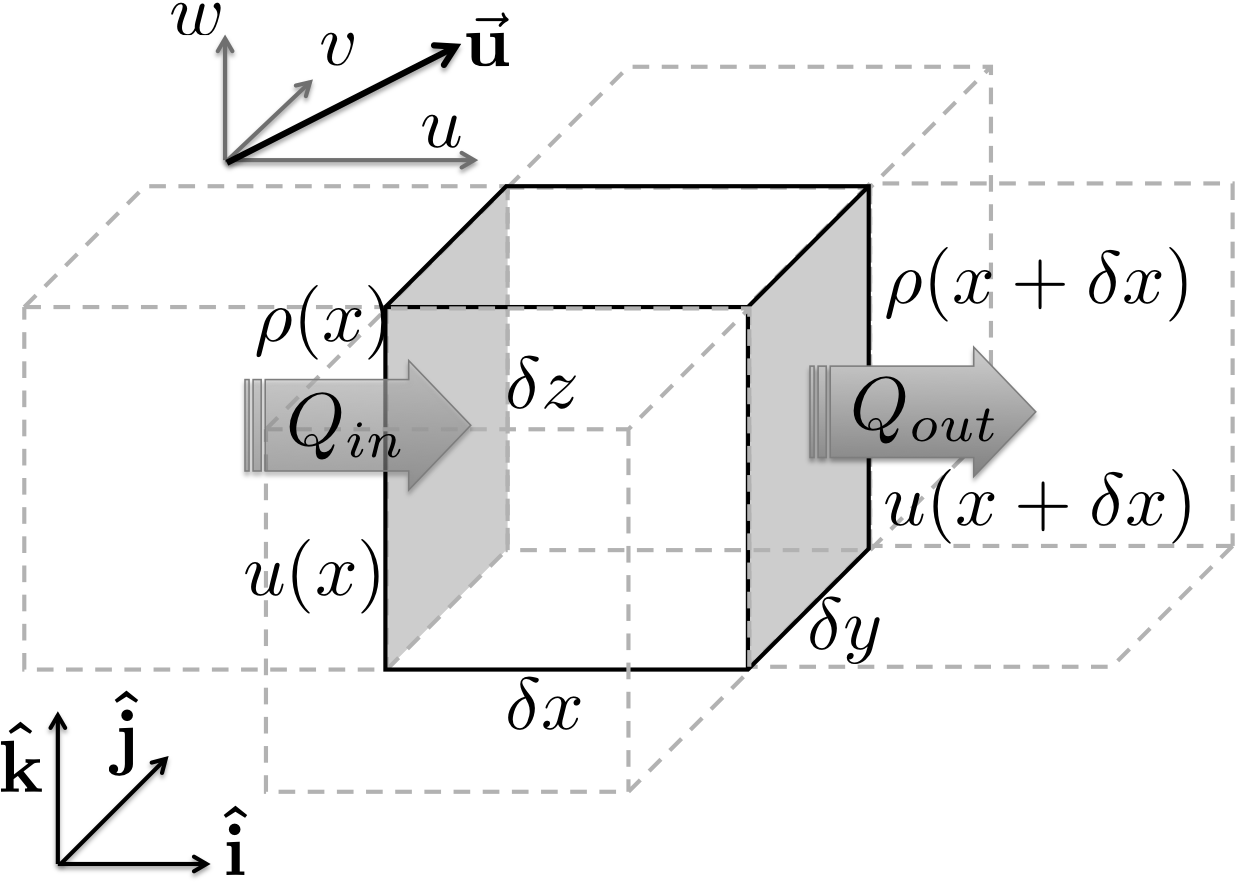
\includegraphics[width=6cm]{../figures/M3/cube_conservation}
\begin{itemize}
\item {\scriptsize{}\vspace{-0.5cm}
The }\textbf{\scriptsize{}local}{\scriptsize{} (Eulerian) time rate
of mass change in the volume is the net flow through all the sides
\begin{align}
\frac{\partial\rho}{\partial t}\,\delta x\,\delta y\,\delta z & =\left(Q_{in}-Q_{out}\right)_{x}+\nonumber \\
 & +\left(Q_{in}-Q_{out}\right)_{y}+\left(Q_{in}-Q_{out}\right)_{z}\label{eq:continuity}
\end{align}
}{\scriptsize\par}
\end{itemize}
\end{columns}

\end{frame}

\begin{frame}{Net mass flow along x}

\begin{itemize}
\item {\small{}The x-component of the net flow is written as 
\[
\left(Q_{in}-Q_{out}\right)_{x}=\rho u\,\delta y\,\delta z-\left[\left(\rho+\delta\rho\right)\left(u+\delta u\right)\right]\delta y\,\delta z
\]
The second term requires some algebra 
\[
\left(\rho u+\rho\delta u+u\delta\rho+\delta\rho\delta u\right)\delta y\,\delta z=\left(\rho u+\rho\frac{\partial u}{\partial x}\delta x+u\frac{\partial\rho}{\partial x}\delta x+\xcancel{\delta\rho\delta u}\right)\delta y\,\delta z
\]
where we used the relationship $\delta u=\frac{\partial u}{\partial x}\delta x$
and $\delta\rho=\frac{\partial\rho}{\partial x}\delta x$ and we ignore
the product of the two small values}{\small\par}
\item {\small{}Going back to the first equation above we can simplify some
terms 
\begin{align}
\left(Q_{in}-Q_{out}\right)_{x} & =\rho u\,\delta y\,\delta z-\rho u\delta y\,\delta z-\left(\rho\frac{\partial u}{\partial x}+u\frac{\partial\rho}{\partial x}\right)\delta x\,\delta y\,\delta z\nonumber \\
 & =-\left(\rho\frac{\partial u}{\partial x}+u\frac{\partial\rho}{\partial x}\right)\delta x\,\delta y\,\delta z\label{eq:Q_x}
\end{align}
}{\small\par}
\end{itemize}
\end{frame}


\section{The continuity equation}
\begin{frame}{The continuity equation}

{\small{}Using eq. (\ref{eq:Q_x}) for the $x$ component and adding
all the other transport terms along $y$ and $z$ in eq. (\ref{eq:continuity}),
we derive the complete form of the continuity equation
\[
\frac{\partial\rho}{\partial t}=-\left(\rho\frac{\partial u}{\partial x}+u\frac{\partial\rho}{\partial x}\right)-\left(\rho\frac{\partial v}{\partial y}+v\frac{\partial\rho}{\partial y}\right)-\left(\rho\frac{\partial w}{\partial z}+w\frac{\partial\rho}{\partial z}\right)
\]
which is rearranged in two forms:}{\small\par}
\begin{enumerate}
\item {\footnotesize{}by recognising the derivative of the product of two
functions in each term between the parentheses:}{\small{}
\begin{equation}
\boxed{\frac{\partial\rho}{\partial t}+\left(\frac{\partial\rho u}{\partial x}+\frac{\partial\rho v}{\partial y}+\frac{\partial\rho w}{\partial z}\right)=0\ \Longrightarrow\ \frac{\partial\rho}{\partial t}+\nabla\cdot\left(\rho\mathbf{u}\right)=0}\label{eq:continuity_equation_rhou}
\end{equation}
}{\small\par}
\item {\footnotesize{}by separating the density and velocity derivatives
and recognising the total derivative and the divergence of velocity:}{\small{}
\begin{align}
\left(\frac{\partial\rho}{\partial t}+u\frac{\partial\rho}{\partial x}+v\frac{\partial\rho}{\partial y}+w\frac{\partial\rho}{\partial z}\right)+\left(\rho\frac{\partial u}{\partial x}+\rho\frac{\partial v}{\partial y}+\rho\frac{\partial w}{\partial z}\right)=0 & \Longrightarrow\boxed{\frac{D\rho}{Dt}+\rho\nabla\cdot\mathbf{u}=0}\label{eq:continuity_equation}
\end{align}
}{\small\par}
\end{enumerate}
\end{frame}


\section{The incompressible ocean}
\begin{frame}{An ocean approximation}

\begin{itemize}
\item The ocean can be approximated to an \emph{incompressible fluid}. We
can assume density does not change much from a reference (constant)
value and spatial and temporal fluctuations are much smaller
\[
\rho=\rho_{0}+\rho^{'}\left(x,y,z,t\right);\ \left|\rho^{'}\right|\ll\rho_{0}
\]
\item All the equations can then be rewritten by separating the terms containing
the constant density and the fluctuation, and neglecting the terms
multiplied by the fluctuation $\rho^{'}$\textbf{
\[
\frac{\left|\rho^{'}\right|}{\rho_{0}}\ll1
\]
}
\item This method was used by Boussinesq to derive a simplified version
of the equation of motion which is used in all modern numerical models
\end{itemize}
\end{frame}

\begin{frame}{An incompressible fluid is non-divergent}

{\footnotesize{}We take one of the forms of the continuity equation
(like eq. (\ref{eq:continuity_equation_rhou}) for instance) and substitute
the density with $\rho=\rho_{0}+\rho^{'}$ 
\[
\frac{\partial\left(\rho_{0}+\rho^{'}\right)}{\partial t}+\left(\frac{\partial\left(\rho_{0}+\rho^{'}\right)u}{\partial x}+\frac{\partial\left(\rho_{0}+\rho^{'}\right)v}{\partial y}+\frac{\partial\left(\rho_{0}+\rho^{'}\right)w}{\partial z}\right)=0
\]
We now divide by $\rho_{0}$
\begin{align*}
\left(\frac{\partial u}{\partial x}+\frac{\partial v}{\partial y}+\frac{\partial w}{\partial z}\right)+\frac{\rho^{'}}{\rho_{0}}\left(\frac{\partial u}{\partial x}+\frac{\partial v}{\partial y}+\frac{\partial w}{\partial z}\right)+\\
+\frac{1}{\rho_{0}}\left(\frac{\partial\rho^{'}}{\partial t}+u\frac{\partial\rho^{'}}{\partial x}+v\frac{\partial\rho^{'}}{\partial y}+w\frac{\partial\rho^{'}}{\partial z}\right) & =0
\end{align*}
and neglect the smaller terms, which are the ones with $\rho^{'}$
derivatives or multiplied by $\rho^{'}$. The equation simplifies
to the notion that }\textbf{\footnotesize{}an incompressible fluid
is non-divergent}{\footnotesize{}
\begin{equation}
\frac{\partial u}{\partial x}+\frac{\partial v}{\partial y}+\frac{\partial w}{\partial z}=\nabla\cdot\mathbf{u}=0\label{eq:div0}
\end{equation}
This equation states that to conserve mass, volume must be conserved. }{\footnotesize\par}
\end{frame}

\begin{frame}{The continuity equation for incompressible fluids}

There is an interesting consideration to be made on the continuity
equation (\ref{eq:continuity_equation})
\[
\frac{D\rho}{Dt}+\rho\nabla\cdot\mathbf{u}=0
\]
\textbf{for the ocean}. Since $\nabla\cdot\boldsymbol{u}=0$ from
eq. (\ref{eq:div0}), the relation states that $\frac{D\rho}{Dt}=0$.
\uline{Be aware that this does not mean that density cannot change.}
The equation implies that \textbf{local density variations} will be
due to the transport of density from the surrounding waters (i.e.
advection), as we can see by expanding the total derivative on the
left hand side of the continuity equation as: 
\[
\underbrace{\frac{\partial\rho}{\partial t}}_{\mathsf{local\,change}}=-\mathbf{u}\cdot\nabla\rho=\underbrace{u\frac{\partial\rho}{\partial x}+v\frac{\partial\rho}{\partial y}+w\frac{\partial\rho}{\partial z}}_{\mathsf{advection\,of\,density}}
\]
\end{frame}

\end{document}
